
\section{Juegos Serios}
\setcounter{sectiontotal}{5}

\begin{frame}
    \frametitle{\pagetitle}
    \framesubtitle{Definición}
    \pause{}
    \begin{block}{Juego Serio}
    \centering
    Es un videojuego que posee un propósito educacional explícito, cuyo objetivo
    principal es el de educar y utiliza conceptos lúdicos para involucrar y
    entretener al usuario
    \end{block}
\end{frame}

\begin{frame}
    \frametitle{\pagetitle}
    \framesubtitle{Características}
     \begin{itemize}[<+->]
         \item Contexto.
         \item Construcción.
         \item Relación con profesionales de la educación.
         \item Nivel cognitivo del alumno.
    \end{itemize}
\end{frame}

\begin{frame}
    \frametitle{\pagetitle}
    \framesubtitle{Ventajas}
    \begin{itemize}[<+->]
        \item Motivación interna
        \item Apoyo al aprendizaje
        \item Menos limitaciones
        \item Similitud a la realidad
        \item Estimulación sensorial
    \end{itemize}
\end{frame}
\note{Mencionar ventajas de las TIC}

\begin{frame}
    \frametitle{\pagetitle}
    \framesubtitle{Desafíos}
	\begin{itemize}[<+->]
        \item Falta de investigación
        \item Expectativas muy altas
        \item Evaluación tradicional
        \item Utilización incorrecta
        \item Falta de recursos
    \end{itemize}
\end{frame}

\begin{frame}
\frametitle{\pagetitle}
\framesubtitle{Áreas de aplicación}

\pause{}
\begin{columns}
\column{.7\textwidth} \hspace{0.5cm}
\begin{itemize}[<+->]
	 \item Militar
     \item Salud
     \item Juegos corporativos
\end{itemize}

\column{.4\textwidth} \hspace{0.5cm}
\begin{overprint}
    \onslide<2|handout:1> 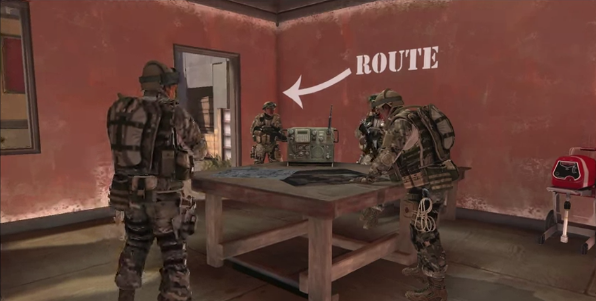
\includegraphics[width=\textwidth, height=4cm]{../tics/images/army} 
    \onslide<3|handout:0> 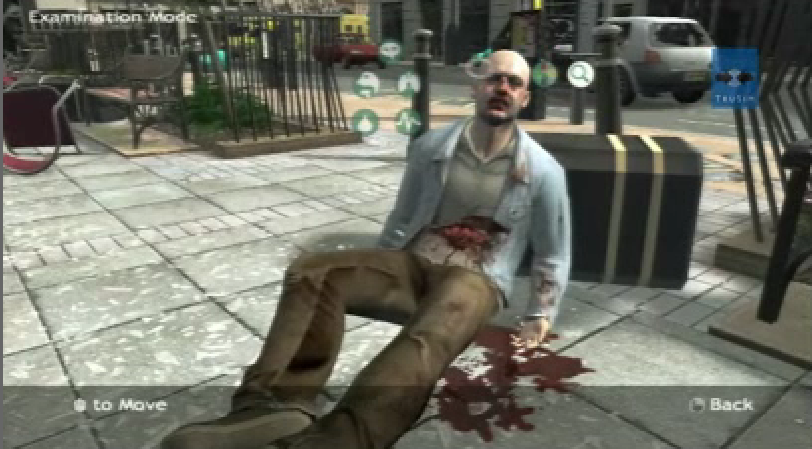
\includegraphics[width=\textwidth, height=4cm]{../tics/images/patient} 
    \onslide<4|handout:0> 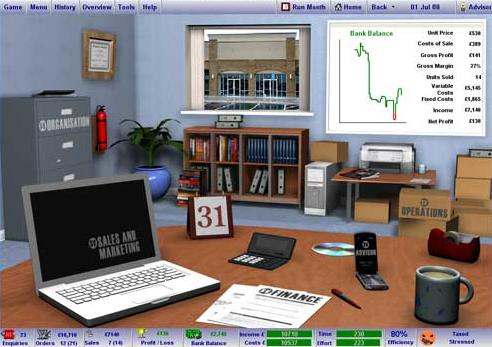
\includegraphics[width=\textwidth, height=4cm]{../tics/images/simventure} 
    
\end{overprint}

\end{columns}


\end{frame}
